\documentclass[heading.tex]{subfiles} 
\begin{document}

\newpage
\appendix

\Appendix{Subsystem Modeling Theory and Potential Future Road Map}

\begin{figure}[hbtp]
\centering
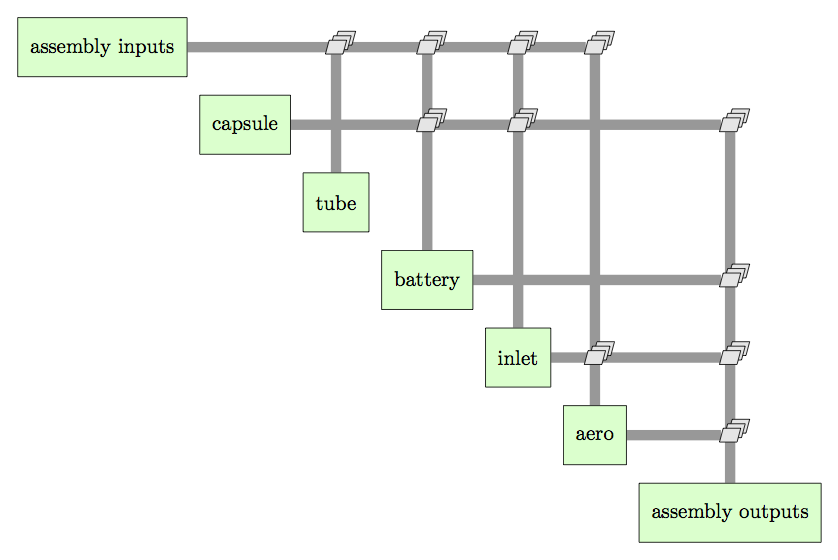
\includegraphics[width=\textwidth]{images/pod_assembly_xdsm.png}
\caption{Expanded \texttt{pod} assembly XDSM}
\label{f:podXDSM}
\end{figure}

\begin{figure}[hbtp]
\centering
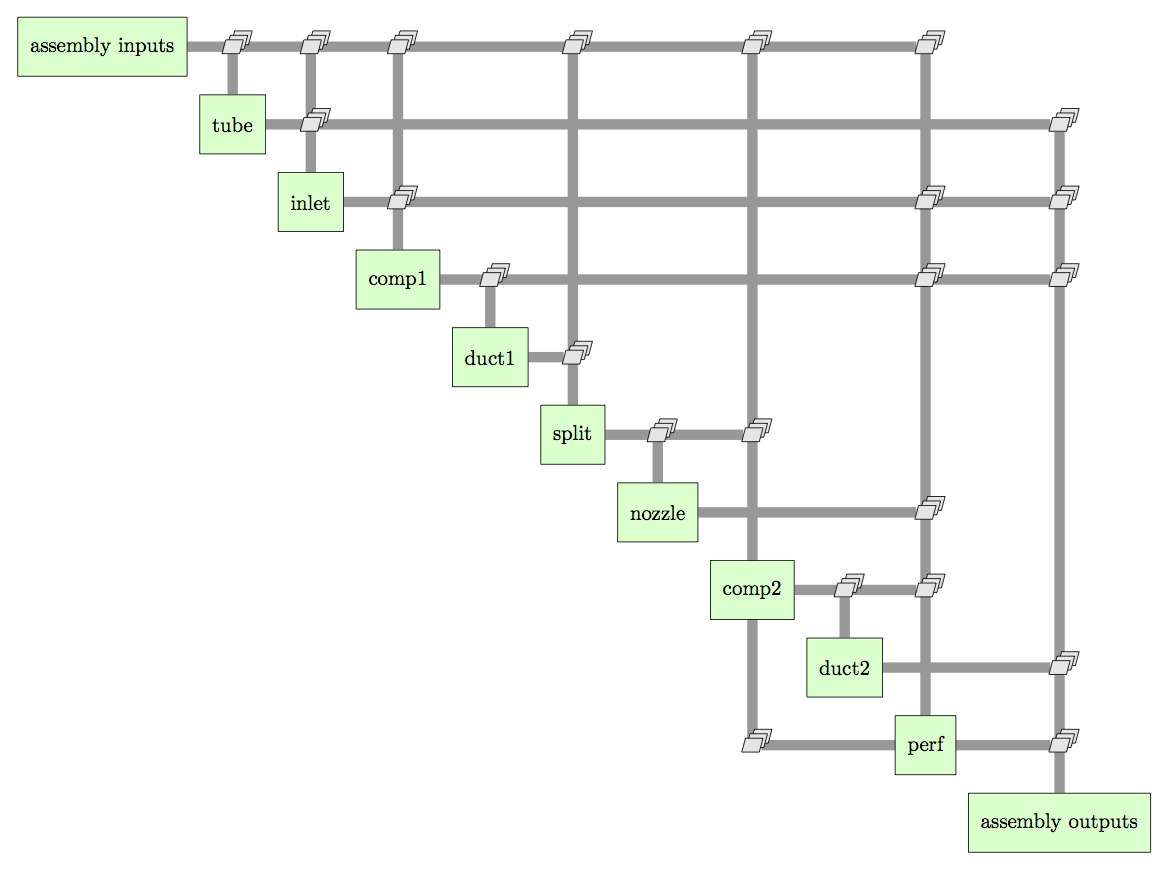
\includegraphics[width=\textwidth]{images/compress_assembly_xdsm.png}
\caption{Expanded \texttt{compress} assembly XDSM}
\label{f:compressorXDSM}
\end{figure}

\subsection{Future Modeling Road Map}

The current model of the hyperloop focuses on some of the primary sub-systems that operate within the pod. However, there is much more
analysis that needs to be done to build a complete hyperloop model.
For the sake of conciseness, each section serves as a general summary. The reader is recommended to refer to the actual source code and
included documentation for full implementation details. The current model omits economic, structural, safety, and infrastructure
considerations; areas that become more prominent once the core engineering concept is deemed sufficiently feasible. These aspects are
equally important to the overall design and they represent the next required step in producing a viable hyperloop design concept.
Below, a brief summary various disciplines are suggested as logical next steps for the engineering aspects of the analysis.

\subsection{System Design Optimization}
The current baseline appears to be a feasible design, but the design space is large (and will grow with additional models) and needs to be
more fully explored. Overall, the goal of the hyperloop design should be to find the right compromise between maximum passenger
throughput, minimum travel time, and minimum cost per trip. The following are some major open questions about the hyperloop design
space:

1) What is the relationship between overall energy usage and tube pressure? Would a slightly higher pressure lower the overall energy
consumption by reducing vacuum pump effort more than it increases power requirements for the pod?

2) What is the best combination of pressure ratios for the compression system? Does the bypass air need to be pressurized so highly?

3) What is the best size for the tube diameter? Larger diameters will increase pump effort, but decrease pod power usage? Could a larger
diameter coupled with a slightly higher pressure provide superior performance?

\subsection{Geometry}
This model makes some simple geometric calculations, however a real parametric geometry model needs to be included. This model is
necessary to properly consider the layout and packaging issues involved in the design, but it also needed to do more complete structural
analyses on the pressurized containers as well as to do an aerodynamic shape optimization of the outer shape.

Some alternate configurations could possibly considered as well. Although the length of the capsule would grow by a factor of almost 2, it
might be possible to put the seats in a single file layout to reduce the overall tube dimensions. The effect of this change on the overall
system is not obvious and needs to be studied.

The geometry model needs to be built in an open source geometry system so that it can be freely shared with the rest of the model.

\subsection{Battery and Motors}
The initial estimates of battery size and weight rely on elementary calculations. As noted, the power requirements amount to roughly
3 to 5 battery packs from a Tesla Model-S. Much better weight and size estimates for these off-the-shelf batteries need to be integrated.

No work has been done to size the motors or account for any cooling requirements they might need. Although the current results indicate
that a cooling system for the compressed air is not needed, it may still be necessary to cool the batteries and motors. The power
requirements, weight, and space needs of such cooling systems needs to be considered.

\subsection{Air Bearings}
The current models assume a fixed mass flow requirement for the air bearing system. A more accurate model would account for the overall
weight of the pod, the pressure of the air, and the overall bearing size. A more detailed bearing model should be coupled to the
compression system model to ensure a feasible design is achieved.

In addition, some investigations need to be made into the lower speed operation of the pod. It's possible that splitting the compression
system into two independent paths would be beneficial, if the bearings require a relatively constant mass flow rate and pressure, because it
would allow a more flexible operation of what is currently the first stage compressor.


\subsection{Vacuum Pumps}
The current model indicates that a tube with around a 4 meter diameter will be needed to reach the high velocities to keep the travel time
to around 35 minutes. The size of the tubes will impact to key power requirements for the vacuum pumps:

The peak power requirements to pump the tubes down in a reasonable time
The steady state power requirements to maintain the high vacuum in the tube
Both of these aspects need to be modeled and incorporated into the system models.


\subsection{Solar Power Generation}
One of the proposed features of the hyperloop concept is its near net-zero energy consumption, via the inclusion of solar panels along the
length of the tubes. Models are needed to predict, based on geographical location, weather, and time of year, how much power could be
produced on an ongoing basis from such a solar panel system.

The power production and power consumption of the hyperloop system need to be compared. Even assuming you can reach a net zero
energy usage on an average basis, the timing of the production and consumption has a strong impact on how much energy storage is
necessary in the overall system. This will have an impact on it's overall cost.

\subsection{Pod Structural Design}
The passenger pod is, from a structural perspective, a pressure vessel experiencing a fairly pressure ratio of around 1000. The original
design concept calls for a non-circular pressure vessel which raises some structural design issues. It's possible to design an effective
structure using modern aircraft grade composites technologies, but it's possible that a round cross section could allow for a more
traditional construction and reduce costs. Structural models considering composites and metallic construction are needed.

\subsection{Component Mass Estimation}
The current model does not include any significant weight estimation. Every part of the model needs to have weight estimates added.

\subsection{Linear Accelerators}
These are not considered at all currently. However, they will obviously need to be modeled as part of the mission analysis work.

\subsection{Route Optimization} \label{app:route}
The current mission analysis takes the velocity profile in the original proposal as a given. We normalize this profile in both time and velocity,
then integrate it. This gives a speed factor of about .8. So for any given maximum velocity, the average velocity would be about 80% of it.

While this simple method provides some basic dependence of travel time on overall speed and tube length it is not really sufficient. A more
advanced analysis needs to be constructed which accounts for actual passenger G-load constraints and can derive an optimal route and
speed profile for a given design.

\begin{figure}[H]
\caption{Velocity profile given in the original proposal}
\centering
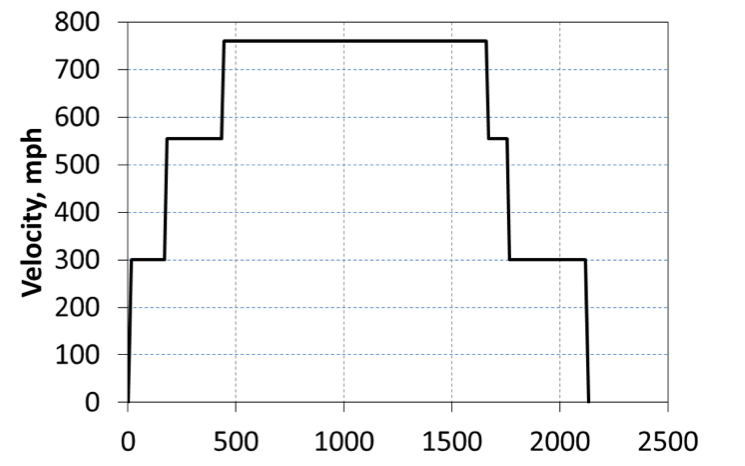
\includegraphics[scale=0.5]{images/velocity_profile.png}
\end{figure}

\subsection{Heat Exchanger Design}

In spite of the results in the capsule cooling section, on-board cooling could possibly be used to partially fulfill cooling requirements. As a
basic exercise a hypothetical baseline heat exchanger model was developed to investigate the weight and sizing requirements of an 
on-board water cooling system using the Logarithmic Mean Temperature Difference (LMTD) method. \cite{Cengal} \cite{Turns} The
exchanger was sized to remove all excess heat generated by the two compressors using a pedagogical shell and tube design. Based on the
temperature restraints and exhaust flow rate determined by the cycle model, necessary water flow rates were calculated to ensure an
energy balance. Given a predefined heat exchanger cross-section, fluid flow regimes and heat transfer coefficients were obtained. The
combination of all of these elements provide a first-cut approximation of tank sizes, total heat exchanger volume, and pumping
requirements.

Given:

-For simplicity, only a single heat exchanger is designed (to cool down the air coming off the first compressor stage)

-Sized as a classic shell and tube heat exchanger

-Input and output temperatures are known for each fluid

-Temperature change across the heat exchanger cannot be so large that Cp changes significantly

-Rigorously defined for double-pipe(or tubular) heat exchanger

With a chosen cross-sectional area of pipe and annulus, and known Q and mdot, the velocity of each fluid can be determined.

\begin{equation*}
\dot{m} = \rho A V     ...therfore...        V  = \frac{Q} {\rho A C_{p} (T_{out} - T_{in})}
\end{equation*}
The hydraulic diameter (characteristic length) of a tube can also be calculated as,
\begin{equation*}
D_{h} = \frac{4 A_{f}} {P_{f}}  = \frac{4 \pi (ID_{a}^2-OD_{p}^2)} {4 \pi (ID_{a}+OD_{p})} = ID_{a}-OD_{p}
\end{equation*}
\begin{equation*}
D_{\varepsilon} = \frac{4 A_{f}} {P_{ht}}   =  \frac{4 \pi (ID_{a}^2-OD_{p}^2)} {4 \pi (ID_{a}*OD_{p})} = \frac{ID_{a}^2-OD_{p}^2}{OD_{p}}
\end{equation*}
Based on the geometry, kinematic viscosity  $\upsilon$ , dynamic viscosity  $\mu$ , thermal conductivity k, and velocity of the fluids the
following non-dimension values can be calculated

Reynolds Number: (inertial forces/ viscous forces)  Re = $\frac{V D_{h}} {\upsilon}$

Prandtl Number: (viscous diffusion rate/ thermal diffusion rate)  Pr = $\frac{C_{p} \mu} {k}$

Based on the flow regimes determined above, the Nusselt Number.. can be calculated. The Dittus-Boelter equation is used in this case,

Nusselt Number: (convective heat transfer / conductive heat transfer)  Nu = $0.023*(Re^{4/5})*(Pr^{n})$ where n = 0.4 if the fluid is heated, n = 0.3 if the fluid is cooled.

Subsequently the convective heat transfer coefficient of each fluid can be determined,  h = $\frac{Nu*k} {D_{\varepsilon}}$

All of these terms can then be used to calculate the overall heat transfer coefficient of the system,

\begin{equation*}
U_{o} = \frac{1} {(\frac{A_{o}}{A_{i}h{i}}) + (\frac{A_{o}ln(\frac{r_{o}}{r_{i}})}{2 \pi k L}) + \frac{1}{h_{o}}}
\end{equation*}
\begin{equation*}
\Delta {T}_{LMTD} = \frac{\Delta {T}_{2}-\Delta {T}_{1}}{ln(\frac{\Delta {T}_{2}}{\Delta {T}_{1}})}
\end{equation*}
\begin{equation*}
\Delta {T}_{1} = T_{hot,in} - T_{cold,out}
\end{equation*}
\begin{equation*}
\Delta {T}_{2} = T_{hot,out} - T_{cold,in}
\end{equation*}
allows the length to be determined for a single pass heat exchanger.
\begin{equation*}
q = U_{o} \pi D_{o} L \Delta {T}_{LMTD}
\end{equation*}
Further calculations for the multipass heat exchanger can be found in the source code.


 \crefalias{section}{appsec}
\Appendix{Sample Source Code and External Contributions} \label{app:2}  

\subsection{Github}

The entire source code can be found on github at:
\url{<https://github.com/OpenMDAO-Plugins/Hyperloop>}

Online documentation can be found at:
\url{<http://openmdao-plugins.github.io/Hyperloop>}

This plugin is designed to be a jumping off point for community contributions to help crowd source the development of the hyperloop
concept. The readme on the github repository walks through basic installation steps, further support can be found through the main
OpenMDAO docs. The basic structure of an assembly is explained in the usage section of these docs.

\subsection{Usage Example}

To use the hyperloop model, you want to run the file src\\hyperloop\\hyperloop\_sim.py in the hyperloop repository. If you have already done that and you're ready to go, then you need not read any farther in this section. We're going to explain whats going on in this file next.

The file starts out with some library imports and the i/o definition of the HyperloopPod assembly.

\inputminted[fontsize=\tiny]{python}{code/example1.py}

Next is the configure method, which is used to wire up the assembly components like the diagrams we show in the model layout section.

First we add an instance of each component class, then connect variables to and from each component.

\inputminted[fontsize=\tiny]{python}{code/example2.py}
 
 Since assemblies often require iteration and convergence, a solver is then added. Each added parameter gives the solver variables to vary, until all declared constraints are satisfied.
%\begin{adjustwidth}{-2cm}{-2cm}
\inputminted[fontsize=\tiny]{python}{code/example3.py}
 %\end{adjustwidth} 
The final ‘’‘if \_\_name\_\_==”\_\_main\_\_”:’‘’ section works the same as you might see it in any other python script. This trick allows the user to set up conditional inputs and parameters for the file to run by itself, rather than in conjunction with the rest of the optimization. Running stand-alone is much more convenient when initially building a component and debugging. 

 %\begin{adjustwidth}{-2cm}{-2cm}
\inputminted[fontsize=\tiny]{python}{code/example4.py} %[linenos]
  %\end{adjustwidth} 

\end{document}